%mainfile: ../master.tex
\chapter{Specification}

This chapter is documentation of the requirement engineering process, as describe in \cite{sommerville}. The structure will follow the elicitation process of requirements, by the methods included in sommerville's book. Some contributing methods used to describe the problem domain are borrowed from \cref{OOAD}. 

Brainstorm of ideas/requirements:
\begin{itemize}
\item The light in a users home will be turned off when not in need for it
\item The light management invisible to the user, light is turned on before a user can observe this behaviour.
\item Will learn usage patterns of the user, turn on light at specific time of day or at a specific light intensity.
\end{itemize}

From the system definition and "rich picture" of the problem domain that the system will be operating, we can extract some classes, \quote{A description of a collection of objects with the same structure, behaviour and attributes}, as described in \cref{OOAD}. This classes will be beneficial when figuring out what we need to keep track of in the problem domain, or what is relevant in our model of the problem domain.

Classes:
\begin{itemize}
\item Person - The user of the system
\item Action - An action the system should recognise as feedback
\item Pattern - The usage patter of a user, what is typical behaviour
\item Mistake - System did something wrong by the user
\item Sensor - The observational member of the system
\item Switch - A feedback source
\item Lamp - The light source on which system action
\item Light intensity - Luminance
\item Room - What room is the user in
\item Premise - The user home enviroment
\item Time - At what time, a pattern property
\end{itemize}

\begin{table}[h!]
\centering
\begin{adjustbox}{max width=\textwidth}
\begin{tabular}{*{15}{|l}|}
    \hline
    \textbf{Event} & Person & Action & Pattern & Mistake & Sensor & Switch & Lamp & Light intensity & Room & Premise & Time \\
    \hline
    Entered home & \cmark & \cmark & \cmark & & \cmark & & \cmark & \cmark & \cmark & \cmark & \\
    \hline
    Left home & \cmark & \cmark & \cmark & & \cmark & & \cmark & & \cmark & \cmark & \\
    \hline
    Enter room & \cmark & \cmark & \cmark & & \cmark & & \cmark & \cmark & \cmark & & \\
    \hline
    Left room & \cmark & \cmark & \cmark & & \cmark & & \cmark & \cmark & \cmark & &\\
    \hline
    Flicked switch & \cmark & \cmark & \cmark & \cmark & \cmark & \cmark & \cmark & \cmark & \cmark & & \\
    \hline
    Outside/External light intensity down & \cmark & & & & \cmark & \cmark & \cmark & \cmark & \cmark & &\\
    \hline
    Outside/External light intensity up & \cmark & & & & \cmark & \cmark & \cmark & \cmark& \cmark & &\\
    \hline
    Person sleeping & \cmark & \cmark & \cmark & & \cmark & & \cmark & & \cmark & & \cmark\\
    \hline
\end{tabular}
\end{adjustbox}
  \caption{Test Table}
  \label{tab:label_test}
\end{table}

%mainfile: ../master.tex
\section{User scenarios}\label{sec:userscenarious}

This section will describe branches of possible narratives derived from the use cases, described in the \cref{sec:usecases}.

\textit{A user is reading a book, the light intensity of the sun is low now due the time of the day, and the user is having trouble reading. The system has learned that at this light intensity when the user is situated at the couch with tv not running, the user now wants the light to be on.}

\textit{A user is home alone in his/her living room. Now leaving a room to go the toilet but does not turn of the light in the living room, while on the toilet the user closes the door and does not observe the light in the living room being turned off by the system to conserve/save energy.}

\textit{A user just left home for a vacation, the user is leaves a few lights on due to stress, the system recognises this and switches the lights off. The user has not been home for 24 hours, the system now initiates in doing short cycles of simulating normal behaviour of the user in some rooms to seed the impression of someone being home, to proactively prevent attracting interest from any observing burglars.}

\textit{In a financial report an organisation recognises a substantial amount of funds is used on lighting the facility. The system generates a report on the lights around the facility, effective lighting hours. Which the supervisors can conclude on to argue were to invest on more energy efficient lighting. Further the system reports on broken or not functioning lighting.}


%Just for fun ? Many users is situated in the living room and the volume(db) of the stereo is really high, so users is shouting to hear each other and this occurs over prolonged duration, the system intellingently lowers the volume without the user noticing. And at 1am/pm(night) the user normally goes to sleep but not today, but because of neighbors the system lowers the volume further.



%mainfile: ../master.tex
\section{Use cases}\label{sec:usecases}

This section will describe ways of interacting with the prototypical system derived from the requirements.

<<<<<<< HEAD
<<<<<<< HEAD
<<<<<<< HEAD
=======
>>>>>>> 9c8f5030b9365c258596d255a2898784b52995cb
\begin{figure}
 \centering 
 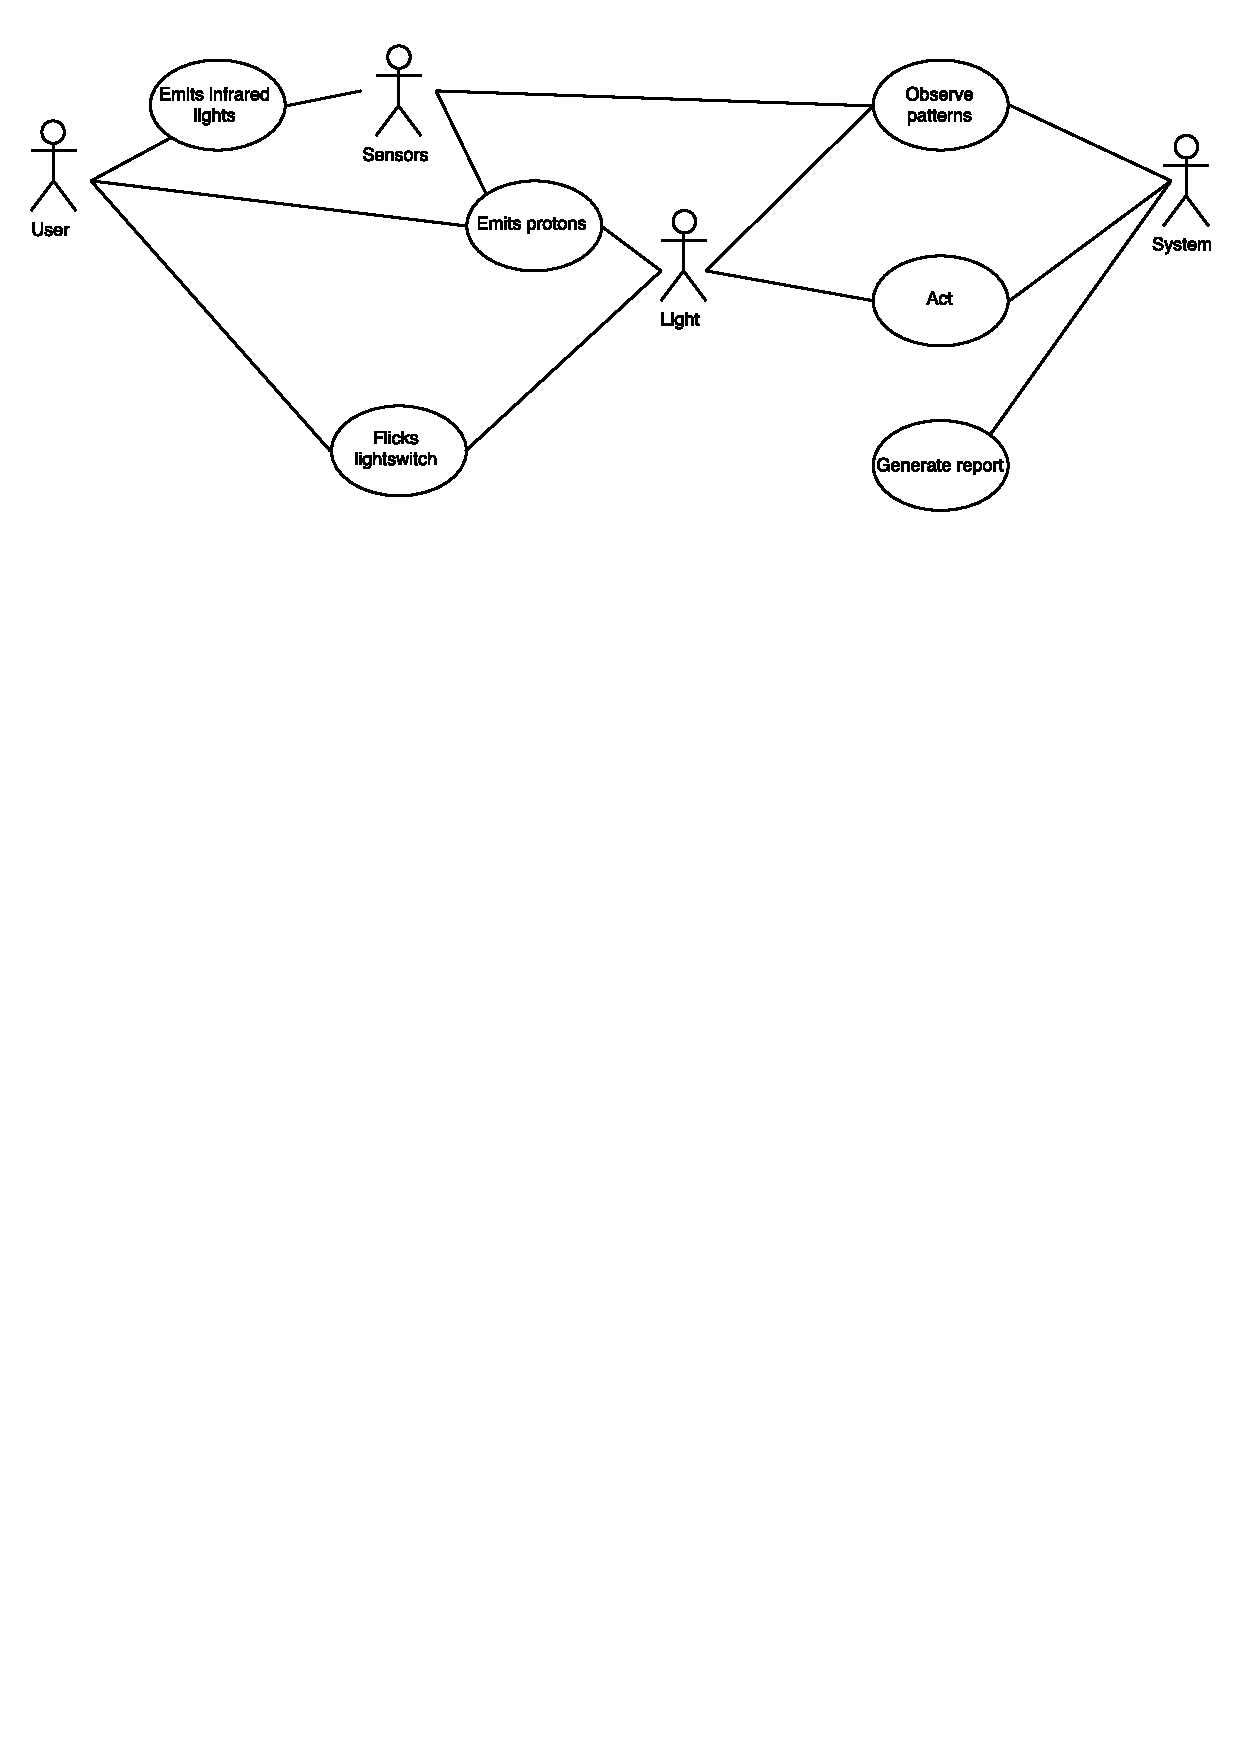
\includegraphics{Usecases.pdf}
 \caption{Rich picture of the problem domain}
\end{figure}
<<<<<<< HEAD
=======

>>>>>>> Specification refactor
=======
\begin{figure}
 \centering 
 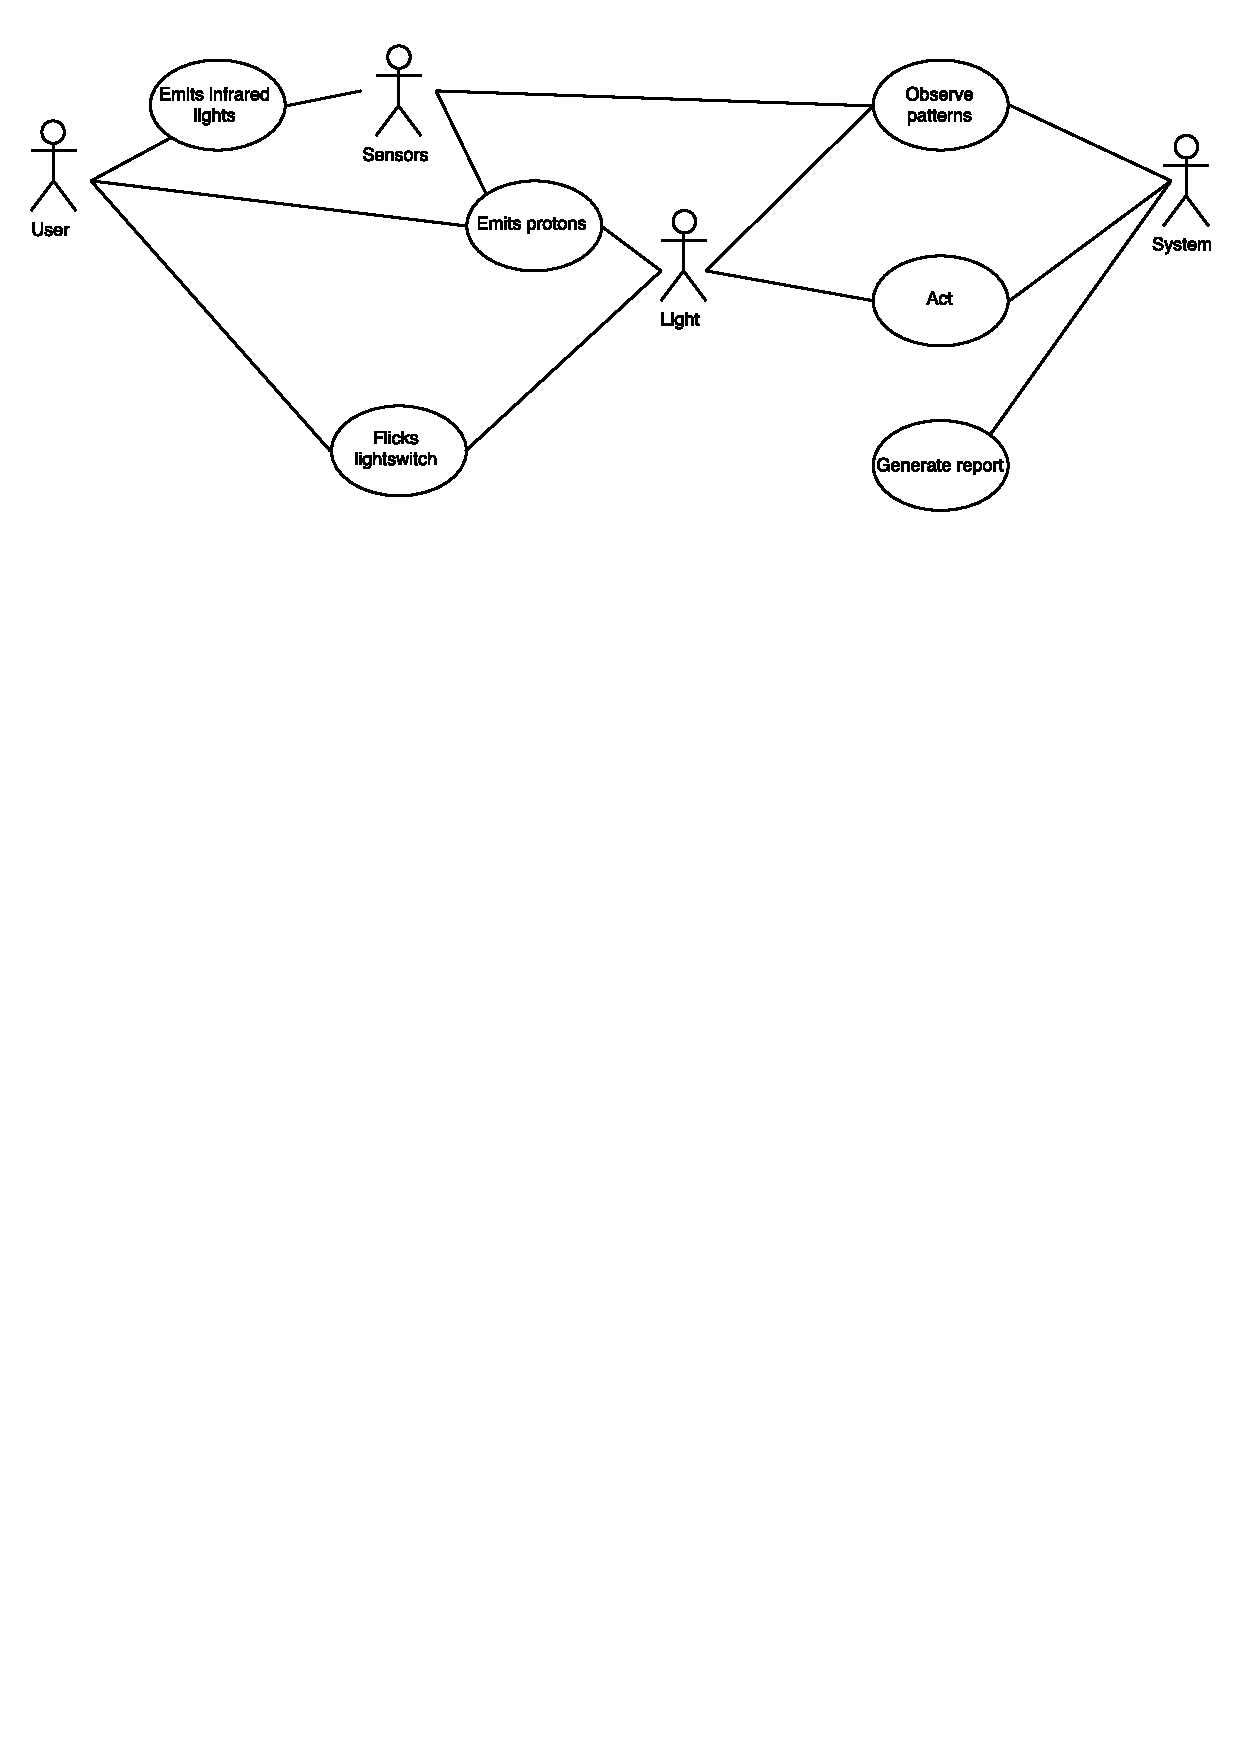
\includegraphics{Usecases.pdf}
\end{figure}
>>>>>>> More user scenarios
=======
>>>>>>> 9c8f5030b9365c258596d255a2898784b52995cb


